% Written By Enoch Yu
% Downloaded from archive.enochyu.com

\documentclass{article}

\usepackage{amsmath}
\usepackage{amsthm}
\usepackage{amssymb}
\usepackage{gensymb}
\usepackage[margin=1in]{geometry}

\usepackage{tikz}
\usetikzlibrary{calc, angles, quotes}
\usepackage{graphicx}
\usepackage{float}
\usepackage[font=small,labelfont=bf]{caption}

\usepackage{parskip}
\usepackage{fancyhdr}
\pagestyle{fancy}
\fancyhead[R]{Enoch Yu}
\pagenumbering{gobble}

\usepackage{enumitem}
\newtheorem{theorem}{Theorem}[section]
\newtheorem{lemma}[theorem]{Lemma}
\newtheorem{sublemma}{Lemma}[section]
\newtheorem{proposition}{Proposition}
\newtheorem{corollary}{Corollary}[theorem]
\newenvironment{solution}{\begin{trivlist}\item[]
{\bf Solution}}{\qed \end{trivlist}}

\pdfinfo{
  /Title (Problem Set 2)
}

\title{Problem Set 2}
\author{Enoch Yu}
\date{29 April 2025}

\begin{document}

\section*{2024 AMC 12B Problem 22}
Let $\triangle{ABC}$ be a triangle with integer
side lengths and the property that
$\angle{B} = 2\angle{A}$. What is the least
possible perimeter of such a triangle?

$\textbf{(A) } 13 \qquad \textbf{(B) } 14 \qquad
\textbf{(C) } 15 \qquad \textbf{(D) } 16 \qquad
\textbf{(E) }17 \qquad$

\begin{solution}

\textbf{Key Word} Law of Sines, Law of Cosines,
Trigonometric Identities, Property of Triangle

\begin{center}
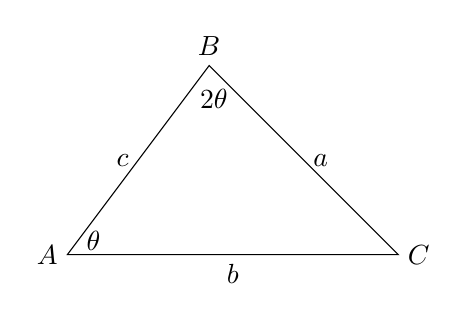
\begin{tikzpicture}[scale=0.6]
    \coordinate (A) at (0,0);
    \coordinate (B) at (3,4);
    \coordinate (C) at (7,0);

    \draw (A) -- (C) -- (B) -- cycle;

    \node[right] at ($(B)!0.5!(C)$) {$a$};
    \node[below] at ($(A)!0.5!(C)$) {$b$};
    \node[left] at ($(A)!0.5!(B)$) {$c$};

    \node at ($(B) + (0.1,-0.7)$) {$2\theta$};
    \node at ($(A) + (0.55,0.3)$) {$\theta$};

    \node[left] at (A) {$A$};
    \node[above] at (B) {$B$};
    \node[right] at (C) {$C$};
\end{tikzpicture}
\end{center}
The fact that $a,b\text{ and }c$ are integers may be utilized.

According to the Law of Sines, the following equation is true.
\begin{align*}
   \frac{b}{\sin{2\alpha}}
   &= \frac{a}{\sin\alpha} \\
   \frac{b}{2 \sin\alpha \cos\alpha}
   &= \frac{a}{\sin\alpha} \\
   \cos\alpha &= \frac{b}{2a}
   \text{ ($\because 0^{\circ} < \alpha < 90^{\circ}$)}
\end{align*}
Moreover, using the Law of Cosines, an additional
equation may be driven.
\[
\cos\alpha = \frac{b^2 + c^2 - a^2}{2bc}
\]
Substitute $\cos\alpha$ to $\cos\alpha = \frac{b}{2a}$.
\begin{align*}
    \frac{b^2 + c^2 - a^2}{2bc} &=\frac{b}{2a} \\
    2a(b^2 + c^2 - a^2) &= 2b^2 c \\
    2ab^2 + 2ac^2 - 2a^3 &= 2b^2 c \\
    2b^2(a-c) + 2a(c^2-a^2) &= 0 \\
    2b^2(a-c) - 2a(a+c)(a-c) &= 0 \\
    (a - c)(2b^2 - 2a(a + c)) &= 0 \\
    (a - c)(2b^2 - 2a^2 - 2ac) &= 0
\end{align*}
Thus, $a - c = 0$ or $2b^2 - 2a^2 - 2ac = 0$ or both
is true. However, when $a = c$, $\alpha = 45^{\circ}$,
which leads to non-integer length for at least one
of the sides.
\begin{align*}
    \therefore 2b^2 - 2a^2 - 2ac &= 0 \\
    b^2 &= a^2 + ac \\
    b^2 &= a(a + c)
\end{align*}
Because the least possible perimeter of such a
triangle must be found, the values for
$a, b \text{ and } c$ could be substituted.
\[
\begin{array}{ccc|cc}
    b & a & c & Validity \\
    \hline
    1 & 1 & 0 & No & \\
    2 & 1 & 3 & No & \text{ }(\because 3 = 2 + 1) \\
    2 & 2 & 0 & No & \\
    3 & 1 & 8 & No & \text{ }(\because 8 > 3 + 1) \\
    3 & 3 & 0 & No & \\
    4 & 1 & 15 & No & \text{ }(\because 15 > 4 + 1) \\
    4 & 2 & 6 & No & \text{ }(\because 6 = 4 + 2) \\
    4 & 4 & 0 & No & \\
    5 & 1 & 24 & No & \text{ }(\because 24 > 5 + 1) \\
    6 & 1 & 35 & No & \text{ }(\because 35 > 6 + 1) \\
    6 & 2 & 16 & No & \text{ }(\because 16 > 6 + 2) \\
    6 & 3 & 9 & No & \text{ }(\because 9 = 6 + 3)\\
    6 & 4 & 5 & Yes & 
\end{array}
\]
Therefore, the least perimeter is $6 + 4 + 5$,
which is \boxed{\text{(C) } 15}.
\end{solution}

\section*{Problem}
In $\triangle{ABC}$, $\angle{B} = 40^{\circ}$ and
$AB + BC = 2AC$. $K$ and $M$ are the mid-points of
$AB$ and $BC$ respectively, while $L$ is a point on
$AC$ such that $BL$ bisects $\angle{ABC}$. Find $\angle{KLM}$.
\begin{solution}

\textbf{Key Word} Angle Bisector Theorem

\begin{center}
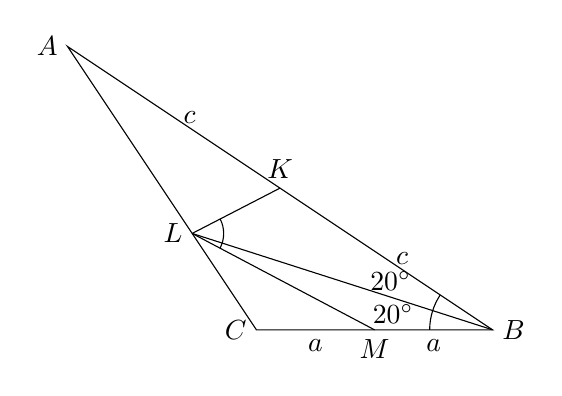
\begin{tikzpicture}[scale=1.2]
    \draw
    (-2,3) coordinate[label=left:$A$] (A) --
    (2.5,0) coordinate[label=right:$B$] (B)  --
    (0,0) coordinate[label=left:$C$] (C) -- cycle;

    \path (B) -- (C) coordinate[pos=0.5] (M);
    \path (A) -- (B) coordinate[pos=0.5] (K);
    \path (A) -- (C) coordinate[pos=0.66] (L);
    \node[below] at (M) {$M$};
    \node[above] at (K) {$K$};
    \node[left] at (L) {$L$};
    \node[below] at ($(C)!0.5!(M)$) {$a$};
    \node[below] at ($(M)!0.5!(B)$) {$a$};
    \node[right] at ($(A)!0.5!(K)$) {$c$};
    \node[right] at ($(K)!0.5!(B)$) {$c$};

    \draw (M) -- (L);
    \draw (L) -- (K);
    \draw (B) -- (L);

    \draw pic["$20^\circ$", draw=black, angle radius=0.8cm,
        angle eccentricity=1.8] {angle=A--B--L};
    \draw pic["$20^\circ$", draw=black, angle radius=0.8cm,
        angle eccentricity=1.6] {angle=L--B--C};
    \draw pic[draw=black, angle radius=0.4cm,
        angle eccentricity=1.6] {angle=M--L--K};
\end{tikzpicture}
\end{center}
According to the problem, $AC = a + c$. Moreover,
using Angle Bisector Theorem, it is evident that
$AL = (a + c) \cdot \frac{c}{a + c}$ and
$LC = (a + c) \cdot \frac{a}{a + c}$.
\begin{center}
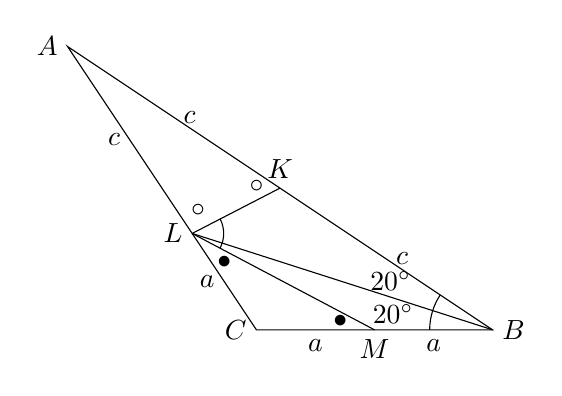
\begin{tikzpicture}[scale=1.2]
    \draw
    (-2,3) coordinate[label=left:$A$] (A) --
    (2.5,0) coordinate[label=right:$B$] (B)  --
    (0,0) coordinate[label=left:$C$] (C) -- cycle;

    \path (B) -- (C) coordinate[pos=0.5] (M);
    \path (A) -- (B) coordinate[pos=0.5] (K);
    \path (A) -- (C) coordinate[pos=0.66] (L);
    \node[below] at (M) {$M$};
    \node[above] at (K) {$K$};
    \node[left] at (L) {$L$};
    \node[below] at ($(C)!0.5!(M)$) {$a$};
    \node[below] at ($(M)!0.5!(B)$) {$a$};
    \node[right] at ($(A)!0.5!(K)$) {$c$};
    \node[right] at ($(K)!0.5!(B)$) {$c$};
    \node[left] at ($(L)!0.5!(C)$) {$a$};
    \node[left] at ($(A)!0.5!(L)$) {$c$};

    \draw (M) -- (L);
    \draw (L) -- (K);
    \draw (B) -- (L);

    \draw pic["$20^\circ$", draw=black, angle radius=0.8cm,
        angle eccentricity=1.8] {angle=A--B--L};
    \draw pic["$20^\circ$", draw=black, angle radius=0.8cm,
        angle eccentricity=1.6] {angle=L--B--C};
    \draw pic[draw=black, angle radius=0.4cm,
        angle eccentricity=1.6] {angle=M--L--K};
    \draw pic["$\circ$", angle eccentricity=0.6]
        {angle=K--L--A};
    \draw pic["$\circ$", angle eccentricity=0.6]
        {angle=A--K--L};
    \draw pic["$\bullet$", angle eccentricity=1.1]
        {angle=C--L--M};
    \draw pic["$\bullet$", angle eccentricity=0.9]
        {angle=L--M--C};
\end{tikzpicture}
\end{center}
Using the property of triangle,
$(180 - 2\circ) + (180 - 2\bullet) = 180 - 40$ is true.
Thereby, $\circ + \bullet = 110$. In another words,
$\boxed{\angle{KLM} = 70^{\circ}}$.
\end{solution}

\newpage
\section*{Problem}
In $\triangle{ABC}$, $AB + BC = 2AC$ and
$\angle{A} = \angle{C} + 90^{\circ}$. Find $\cos{B}$.

\subsection*{Solution I}
\begin{minipage}{0.5\textwidth}
\textbf{Key Word} Law of Sines, Law of Cosines
\begin{center}
\begin{tikzpicture}[scale=1.4]
    \draw
        (-2,3) coordinate[label=left:$C$] (A) --
        (2.5,0) coordinate[label=right:$B$] (B)  --
        (0,0) coordinate[label=left:$A$] (C) -- cycle;

    \node[below] at ($(C)!0.5!(B)$) {$c$};
    \node[right] at ($(A)!0.5!(B)$) {$a$};
    \node[left] at ($(C)!0.5!(A)$) {$\frac{a + c}{2}$};

    \draw pic["$\theta$", draw=black, angle radius=0.8cm,
        angle eccentricity=1.2] {angle=C--A--B};
    \draw pic["$90^{\circ} + \theta$", draw=black,
        angle radius=0.2cm, angle eccentricity=3] {angle=B--C--A};
\end{tikzpicture}
\end{center}
\end{minipage}
\begin{minipage}{0.5\textwidth}
A vertical line from $A$ could be drawn.
\begin{center}
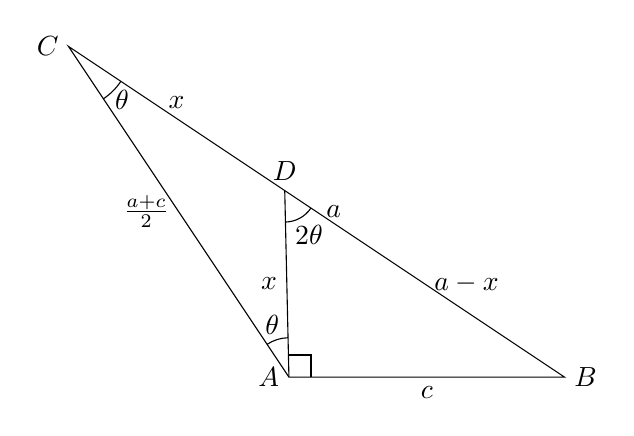
\begin{tikzpicture}[scale=1.4]
    \draw
        (-2,3) coordinate[label=left:$C$] (A) --
        (2.5,0) coordinate[label=right:$B$] (B)  --
        (0,0) coordinate[label=left:$A$] (C) -- cycle;

    \path (A) -- (B)
        coordinate[pos=0.436, label=above:$D$] (D);

    \node[below] at ($(C)!0.5!(B)$) {$c$};
    \node[right] at ($(A)!0.5!(B)$) {$a$};
    \node[left] at ($(C)!0.5!(A)$) {$\frac{a+c}{2}$};
    \node[left] at ($(C)!0.5!(D)$) {$x$};
    \node[above] at ($(A)!0.5!(D)$) {$x$};
    \node[above, right] at ($(D)!0.5!(B)$) {$a-x$};

    \draw (C) -- (D);

    \draw (0, 0.2) -- (0.2, 0.2) -- (0.2, 0);

    \draw pic["$\theta$", draw=black, angle radius=0.8cm,
        angle eccentricity=1.2] {angle=C--A--B};
    \draw pic["$\theta$", draw=black, angle radius=0.5cm,
        angle eccentricity=1.4] {angle=D--C--A};
    \draw pic["$2\theta$", draw=black, angle radius=0.4cm,
        angle eccentricity=1.6] {angle=C--D--B};
\end{tikzpicture}
\end{center}
\end{minipage}

$\cos(90^{\circ} - 2\theta)$, or $\sin2\theta$,
is the value that is required to be computed.
According to the diagram, it is evident that
$\sin2\theta = \frac{c}{a - x}$.

To compute the value of $x$, trigonometric
identities may be utilized.
$\tan2\theta = \frac{2\tan\theta}{1 - \tan^2\theta}$
is true.

The Law of Sines may provide additional information.
\[
\frac{\frac{a + c}{2}}{\sin(90 - 2\theta)}
= \frac{c}{\sin\theta} = \frac{a}{\sin(90 + \theta)}
\]
In another words,
\begin{align*}
    \frac{c}{\sin\theta} &= \frac{a}{\cos\theta} \\
    \frac{c}{a} &= \frac{\sin\theta}{\cos\theta} \\
    \tan\theta &= \frac{c}{a}
\end{align*}
Because $\tan2\theta = \frac{2\tan\theta}{1 - \tan^2\theta}$,
$\frac{c}{x} = \frac{2\cdot\frac{c}{a}}{1 - (\frac{c}{a})^2}$.
\begin{align*}
    a - x &= a - c\cdot
        \frac{ 1 - (\frac{c}{a})^2 }{ 2\cdot\frac{c}{a} } \\
    &= a - (1 - \frac{c^2}{a^2}) \cdot
        \frac{c}{ 2 \cdot \frac{c}{a} } \\
    &= a - (1 - \frac{c^2}{a^2}) \cdot \frac{a}{2} \\
    &= \frac{a}{2}
        \left(2 - \left( 1 - \frac{c^2}{a^2} \right) \right) \\
    &= \frac{a}{2} \left(1 + \frac{c^2}{a^2} \right) \\
    &= \frac{a}{2} \left( \frac{a^2 + c^2}{a^2} \right) \\
    &= \frac{a^2 + c^2}{2a}
\end{align*}
Therefore, the value of
$\sin2\theta = \frac{c}{\frac{a^2 + c^2}{2a}}
= \frac{2ac}{a^2 + c^2}$.

The Law of Cosines may provide supplementary information.
\begin{align*}
    \cos\theta &=
        \frac{ a^2 + (\frac{a + c}{2})^2 - c^2 }
            { 2\cdot a \cdot \frac{a + c}{2} } \\
    \cos(90 + \theta) &=
        \frac{ c^2 + (\frac{a + c}{2})^2 - a^2 }
            { 2 \cdot c \cdot \frac{a + c}{2} }
        = -\sin\theta
\end{align*}
Using the fact $\tan\theta = \frac{c}{a}$ again,
the following equations may be written.
\begin{align*}
    \frac{c}{a}
    &= \frac{ \frac{ a^2 - (\frac{a + c}{2})^2 - c^2 }
            { 2 \cdot c \cdot \frac{a + c}{2} } }
            { \frac{ a^2 + (\frac{a + c}{2})^2 - c^2 }
            { 2 \cdot a \cdot \frac{a +c }{2} } } \\
    &= \frac{ \frac{a^2 - (\frac{a + c}{2})^2 - c^2}{c}}
        { \frac{ a^2 + (\frac{a + c}{2})^2 - c^2}{a} } \\
    \frac{c^2}{a^2}
    &= \frac{a^2 - c^2 - (\frac{a + c}{2})^2}
        {a^2 - c^2 + (\frac{a + c}{2})^2} \\
    c^2 \left( a^2 - c^2 + (\frac{a + c}{2})^2 \right)
    &= a^2 \left( a^2 - c^2 - (\frac{a + c}{2})^2 \right) \\
    a^2 c^2 - c^4 + \frac{c^2}{4} (a + c)^2
    &= a^4 - a^2 c^2 - \frac{a^2}{4}(a + c)^2 \\
    c^2 (a^2 - c^2) + \frac{c^2}{4} (a + c)^2
    &=a^2 (a^2 - c^2) - \frac{a^2}{4}(a + c)^2 \\
    c^2 (a - c) + \frac{c^2}{4} (a + c)
    &=a^2(a - c) - \frac{a^2}{4}(a + c) \\
    \frac{c^2}{4} (a + c) + \frac{a^2}{4} (a + c)
    &= a^2(a - c) - c^2(a - c) \\
    (a + c) ( \frac{c^2}{4} + \frac{a^2}{4} )
    &= (a - c)(a^2 - c^2) \\
    ( \frac{c^2}{4} + \frac{a^2}{4} )
    &= (a - c)(a - c) \\
    c^2 + a^2 &= 4a^2 - 8ac + 4c^2 \\
    3a^2 + 3c^2 &= 8ac \\
    \frac{2ac}{a^2 + c^2} &= \frac{3}{4} \\
\end{align*}
$\therefore \sin2\theta = \boxed{\frac{3}{4}}$.

\newpage
\subsection*{Solution II}
\textbf{Key Word} Trigonometric Identities, Law of Sines
\begin{center}
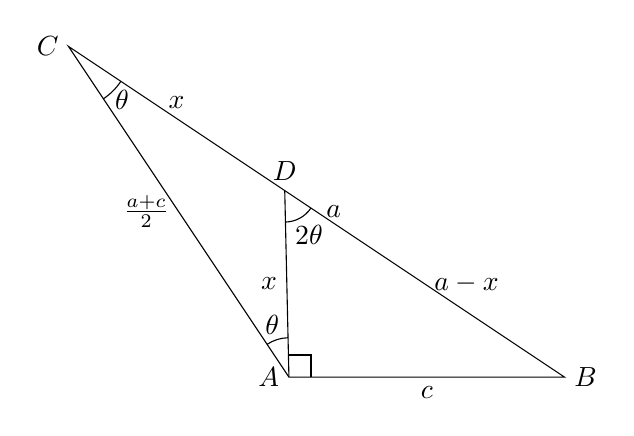
\begin{tikzpicture}[scale=1.4]
    \draw
        (-2,3) coordinate[label=left:$C$] (A) --
        (2.5,0) coordinate[label=right:$B$] (B)  --
        (0,0) coordinate[label=left:$A$] (C) -- cycle;

    \path (A) -- (B) coordinate[pos=0.436, label=above:$D$] (D);

    \node[below] at ($(C)!0.5!(B)$) {$c$};
    \node[right] at ($(A)!0.5!(B)$) {$a$};
    \node[left] at ($(C)!0.5!(A)$) {$\frac{a+c}{2}$};
    \node[left] at ($(C)!0.5!(D)$) {$x$};
    \node[above] at ($(A)!0.5!(D)$) {$x$};
    \node[above, right] at ($(D)!0.5!(B)$) {$a-x$};

    \draw (C) -- (D);

    \draw (0, 0.2) -- (0.2, 0.2) -- (0.2, 0);

    \draw pic["$\theta$", draw=black, angle radius=0.8cm,
        angle eccentricity=1.2] {angle=C--A--B};
    \draw pic["$\theta$", draw=black, angle radius=0.5cm,
        angle eccentricity=1.4] {angle=D--C--A};
    \draw pic["$2\theta$", draw=black, angle radius=0.4cm,
        angle eccentricity=1.6] {angle=C--D--B};
\end{tikzpicture}
\end{center}
From the diagram above, the Law of Sines could be used.
\[
\frac{c}{\sin\theta} = \frac{a}{\sin(90 + \theta)}
= \frac{ \frac{a + c}{2} }{ \sin B }
= \frac{a + c}{ \sin\theta + \sin(90 + \theta) }
\]
In another words,
\begin{align*}
    2 \sin B &= \sin\theta + \sin(90 + \theta)
        =2 \sin\frac{ \theta + (\theta + 90)}
            {2} \cos\frac{ \theta - (\theta + 90) }{2} \\
    &=4\sin{\frac{B}{2}}\cos{\frac{B}{2}}
\end{align*}
Therefore,
\begin{align*}
    4 \sin{\frac{B}{2}} \cos{\frac{B}{2}}
    &= 2 \sin\frac{ \theta + (\theta + 90)}{2}
        \cos\frac{ \theta - (\theta + 90) }{2} \\
    &= 2 \sin\frac{ 2\theta + 90}{2} \cos45^{\circ} \\
    &=\sqrt{2} \cos\frac{B}{2} \\
    4 \sin\frac{B}{2}
    &= \sqrt{2} \\
    \sin\frac{B}{2}
    &= \frac{ \sqrt{2} }{4} \\
    \sqrt{ \frac{1 - \cos B}{2}}
    &= \frac{ \sqrt{2} }{4} \\
    \frac{ 1 - \cos B }{2}
    &= \frac{1}{8} \\
    \therefore \boxed{\cos B = \frac{3}{4}}
\end{align*}
\end{document}

